% !Mode:: "TeX:UTF-8"

\chapter[绪论]{绪论}[]

\section{研究背景及意义}

\subsection{研究背景}

深度神经网络在计算机视觉领域的诸多基准任务上取得了令人瞩目的成绩，ImageNet、COCO 等大规模标注数据上的识别精度接近甚至超越人类水平，但其性能突破的背后隐含着一个常被忽视的前提：训练数据与测试数据服从独立同分布~\cite{liang2021source}。在真实部署中，目标侧条件偏离训练条件的方式并非单一维度，而是同时在数据分布、类别词表、语义层次三个维度上发生偏移，由此引发三类在抽象层次上逐级递进的稳健性问题。如图~\ref{fig:iidood}所示，传统独立同分布训练假设下的模型在上述任一维度发生偏移时都会出现明显的性能退化。

\begin{figure}[!htbp]
 \centering
 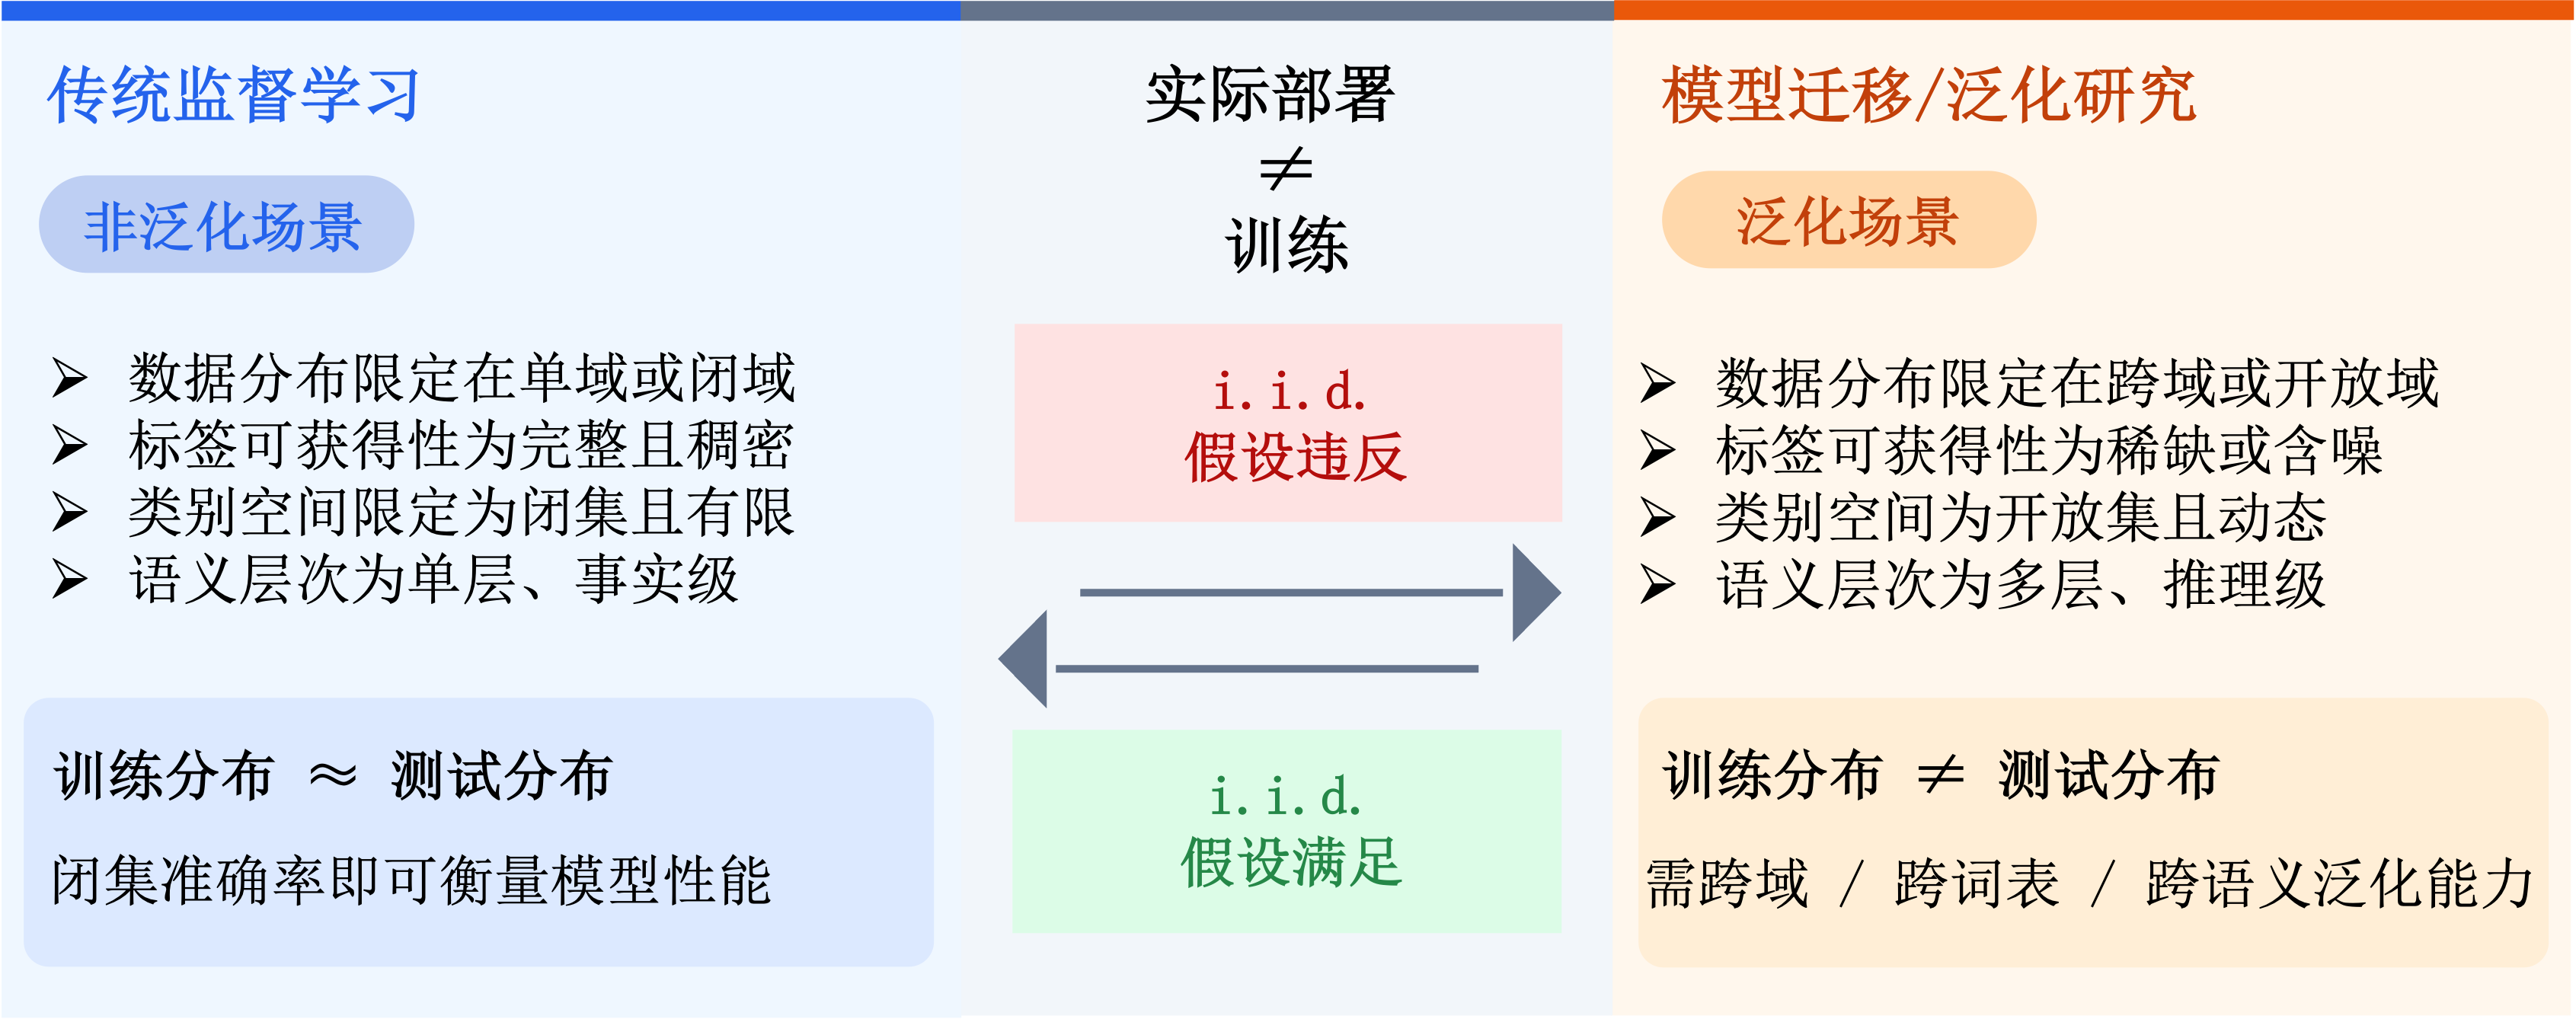
\includegraphics[width=1.\linewidth]{figures/iidood.png}
 \bicaption[fig:iidood]{}{传统独立同分布（i.i.d.）训练假设与多泛化场景的多维对比}{Fig.}{Comparison of traditional i.i.d. training assumption and multi-domain generalization scenarios}
\end{figure}

数据分布维度的失配是最直观且被研究最为广泛的一类稳健性问题。深度神经网络在训练过程中习得的并非纯粹的类别语义表征，而是将语义信息与源域的纹理风格、光照条件、采集设备特征等多层次信息深度纠缠地编码于同一特征空间~\cite{ganin2016domain,long2015learning}。这种纠缠根源于经验风险最小化在 i.i.d. 假设下对源域损失的直接优化。过参数化的网络倾向于记忆源域样本的表面统计而非学习真正可泛化的语义不变特征，使得跨域时分类器权重所定义的判别方向在源域最优而在目标域系统性偏移。这种偏移进一步导致模型在目标域的预测不仅精度下降，还伴随显著的高置信度错误风险，例如softmax 输出对未知样本仍给出接近 1.0 的伪置信，使决策难以被阈值过滤或人工干预~\cite{liang2021source,yang2021neighbor}。在更严苛的无源设定下，源域数据因隐私法规、商业机密或存储成本等约束不可访问，模型需在源数据完全缺位的条件下仅凭源模型参数中编码的知识完成跨域传递，而由于深度特征的纠缠本质，我们无法从模型参数中直接辨识哪些知识可迁移、哪些是源域特定的虚假相关，进一步加剧了迁移的不确定性，所以就需要结合目标域数据进一步做不确定分析。
本文将这种需要将模型部署到数据分布偏移的场景称之为“域泛化”场景，与文献~\cite{zhou2023domain}中特指模型在源域完成泛化而部署时完全不接触任何目标数据的域泛化设定在前提假设上并不等同。

类别词表维度的失配是另一类广泛存在却长期被低估的稳健性问题。传统深度分类器在架构层面预设了闭集假设，即分类头的输出维度等于训练类别数，其判别性表征也是在固定类别索引上优化得到的~\cite{radford2021learning}。这一架构选择带来双重约束：一方面，分类头的权重矩阵与固定的 N 个类别索引强绑定，新类别没有对应的输出通道；另一方面，骨干网络针对 N 类判别任务优化，并未在特征空间中为未知类别预留结构化空间~\cite{kundu2022towards}。当目标场景的类别集合发生扩展、缩减或漂移时，分类头的维度结构与新类别空间在维度上不再兼容，已训练模型的判别能力在新类别上无法直接复用，并倾向于将未知样本强行归入概率最高的已知类别，产生高置信度的错误预测。这一现象在自动驾驶、工业质检等在线服务场景中尤为危险~\cite{kirillov2023segment}。为缓解这一约束，基于图文对比预训练的开放词汇分类器通过引入语言空间的语义先验扩展了类别边界，但其语义覆盖仍受限于预训练文本编码器的词表，难以覆盖长尾、新兴或专业领域类别~\cite{radford2021learning}。逐类重新采集、专家标注并重训模型的过程伴随显著的时间与资金投入，在隐私敏感与不可中断的业务场景中，这种``重训窗口''往往根本不可行~\cite{kirillov2023segment}。这要求识别模型能够在训练时未见过的新类别上完成判别，而传统固定词表架构在维度不兼容的设定下难以直接扩展，尤其在像素级分割任务中，新类别的精细空间定位对像素级标注成本与模型先验的开放语义能力同时提出要求，使类别词表维度的失配在通用识别研究中成为一个关键挑战。

语义层次维度的失配是相较前两者更高阶的稳健性问题。现有视觉基础模型（特别是多模态大语言模型）的预训练以事实型图文描述为主，习得的表征擅长回答“图像中有什么”这类可枚举的类别问题~\cite{mmbench2023}，却对隐含于视觉元素与文化语境、风格表征、符号解读之间的关联缺乏结构化编码，其流畅的语义表述多源于训练语料的统计相关而非基于视觉证据的可靠推理~\cite{achlioptas2021artemis,zhao2014exploring}。具体而言，预训练语料中的图像描述通常以物体、场景、动作等可枚举事实为骨架，而高阶情感与文化推理所需的细粒度证据化标注（如“左上方冷色笔触营造孤寂氛围”）在大规模数据中极为稀缺~\cite{aesexpert2024}，导致模型缺乏从局部视觉元素到整体情感语义的可追溯推理路径，其生成结果常表现为“流畅的虚构”——语言流畅、符合人类表达习惯，但缺乏对具体视觉元素的精确指涉~\cite{eemobench2025}。当识别任务从事实判断升级到“图像为何传达某种情感”、“差异由哪些视觉线索驱动”等需要感知能力与文化语境相融合的高阶推理时，模型所依赖的不再是可枚举的类别标签或显式物体事件，而是隐含在视觉元素与文化符号之间的语义关联。以艺术图像的情感推理为例，情感表达隐含于构图、笔触、风格化与文化符号之中，不同艺术流派的笔触技法与色彩配置所引发的情感反应具有显著的领域特异性~\cite{yang2023emoset}。然而现有通用多模态大语言模型评测基准多聚焦于事实识别层面~\cite{mmbench2023}，缺乏面向情感理解与证据化推理的结构化诊断协议，使得流畅的情感表述与基于视觉证据的可靠解释难以被精准区分~\cite{eemobench2025}，阻碍了视觉基础模型在高阶语义推理方向上的能力迭代。

综上，本文将训练条件与实际部署条件不一致所引发的模型稳健性问题概括为多泛化场景。模型迁移的目标并不止于将模型参数或表征从训练环境带入目标环境，更在于验证其能力能否在新的数据、任务与认知要求下稳定延续；当目标侧缺乏可用于再训练的监督信息时，系统化评测便成为刻画和诊断迁移效果的重要机制。基于此，多泛化场景可由三个相互关联的要素刻画。其一，偏移维度描述训练与部署之间发生变化的对象，包括数据分布、类别词表与语义层次三类失配。其二，资源约束描述目标侧可获得监督信息的程度，涵盖完全无标注、少量人工标注和纯评测三种形态。其三，迁移载体描述承载与传递知识的模型形式，主要包括判别式视觉模型与多模态大语言模型（Multimodal Large Language Model, MLLM）。三类要素共同决定了模型需要迁移何种知识、能够利用何种监督，以及应采用何种学习或评测机制。

围绕上述多泛化场景，本文沿域泛化、类泛化与语义理解泛化三个层面展开研究。域泛化以数据分布变化为核心，面向判别式视觉模型在无标注或少量标注条件下的可靠迁移：前者通过伪标签去噪和鲁棒表征学习抑制迁移过程中的误差累积，后者利用多模态先验引导主动样本选择，以有限标注获得更高效的适应收益。类泛化进一步关注类别词表的开放变化，在无标注条件下结合多模态先验与多基础模型协同，突破固定词表对新颖类别识别和像素级定位的限制。语义理解泛化则面向语义层次提升，以 MLLM 为迁移载体，在纯评测条件下构建多层级、多维度的评测协议，系统诊断其在情感理解、证据关联与高阶推理等任务中的能力边界。


\subsection{研究意义}
多泛化场景下的模型迁移并非由彼此独立的挑战构成，而是呈现出由低到高、逐层递进的稳健性需求。数据分布维度关注像素风格、成像条件与统计特性的变化，核心在于学习具有跨域稳定性的表征；类别词表维度关注模型对未见类别的语义覆盖能力，核心在于实现开放环境下的识别与泛化；语义层次维度关注模型能否超越事实层面的对象判别，完成情感归因、证据关联与高阶推理。
三类挑战在实际任务中具有明显的传导关系。不稳定的跨域表征会削弱开放类别识别的可靠性，而有限的类别语义覆盖又会限制模型开展更高层次语义理解与推理。因此，模型迁移需要沿着“表征—概念—语义”的路径逐层推进。这一递进关系为本文各章工作提供了统一主线，也为复杂开放环境下模型训练策略与评测范式的设计提供了理论参照。

\noindent\textbf{（1）域泛化方面} 

模型能否将训练阶段获得的知识有效迁移至分布不同的目标域，是迁移学习长期关注的核心问题~\cite{liang2021source,ganin2016domain,long2015learning}。棘手的是，深度表征中所蕴含的可迁移成分与域特异性成分在缺乏显式分解机制的条件下彼此纠缠，仅靠目标域自监督信号难以可靠地区分二者，伪标签噪声放大与判别性偏移是这一困境在方法层面的集中体现~\cite{yang2021neighbor,kundu2022towards}。同时，受数据隐私、版权保护和传输成本等现实因素影响，源域样本往往难以获取，使迁移过程中的可靠性诊断更具挑战。因此，研究源数据受限乃至不可访问条件下的可靠迁移机制，一方面有助于深化对无源域适应和少监督域适应中伪标签去噪、有效样本选择与鲁棒表征学习机制的认识；另一方面也能够为面向真实部署环境的目标域特征学习与高效适应策略提供方法依据。

\noindent\textbf{（2）类泛化方面} 

视觉识别系统在实际应用中面对的不再是封闭且预定义的类别集合，而是持续扩展的开放词汇空间。新物体、新材质、新场景不断涌现，固定训练词表及其对应的分类决策边界班一覆盖开放环境中的识别需求~\cite{kirillov2023segment,radford2021learning}。当模型遭遇训练阶段未见的类别时，往往会将其错误归入已有类别，并产生高置信度预测~\cite{kundu2022towards}。由此，开放词汇视觉识别的关键在于缓解封闭训练词表与开放识别需求之间的结构性错配。研究如何在缺乏目标类别标注的条件下发挥多模态基础模型的开放语义先验，并构建异质模型之间的协同机制，有助于揭示语义知识与空间定位知识的互补规律。这不仅能够为开放词汇分类、检测和分割模型的设计提供方法支撑，也有望降低模型适应新类别时对大规模重新训练和人工标注的依赖。

\newpage
\noindent\textbf{（3）语义理解泛化方面} 

多模态大语言模型已在多类事实型视觉识别任务中展现出较强能力，但在情感、意图、文化语境和审美判断等高阶语义任务中，其能力边界仍有待系统刻画~~\cite{mmbench2023,achlioptas2021artemis,eemobench2025}。这一挑战的深层原因在于：模型的预训练语料以可枚举的事实型图文描述为主，缺乏将局部视觉元素与整体情感语义相连接的可追溯推理路径~\cite{zhao2014exploring,aesexpert2024}；其语言流畅性往往源于训练统计相关而非视觉证据支撑~\cite{eemobench2025}。构建面向高阶视觉语义的标准化评测协议，是模型迁移研究在纯评测条件下的重要延伸：当目标任务缺少可用于进一步训练的监督信息时，评测能够刻画和诊断模型既有知识能否有效迁移至新的语义理解任务。此类评测不仅可为多模态大语言模型的能力诊断和后续优化提供量化依据，也有助于揭示视觉智能从感知走向认知仍然缺失的关键能力，从而推动视觉基础模型向更可靠、更具证据支撑的高阶语义推理发展。将高阶语义理解沿感知、情感、推理与描述四个多维互补层级分别考察，使语义层面的能力边界既可被定位也可被比较。

\section{国内外研究现状}

\subsection{面向样本实例的跨域不变特征学习}

在真实场景中，模型所提取的视觉表征不可避免地需要在多种分布条件下保持稳定。光照强度与色温的变化、采集设备与拍摄视角的差异、图像风格与渲染方式的切换，都会使同类目标在像素空间呈现出截然不同的统计形态，而人类视觉系统对此类变化具有天然的判别鲁棒性。赋予模型类似的跨域稳定性，是域适应研究希望达成的根本目标：学习能够抵御分布偏移、对目标类别保持判别力的视觉表征。本节关注样本实例层面的跨域不变性：在视觉外观因光照、风格、采集设备等发生显著变化时，判别性特征仍能被稳定提取的能力。如何系统地实现这一目标，是域不变特征学习所面临的核心任务，其本质在于从模型参数中分解出具有跨域迁移能力的语义成分，同时抑制与特定数据分布耦合的域相关成分。从技术构成看，跨域不变特征学习由两条相互正交的设计维度共同决定：方法范式设计跨域不变性学习机制；骨干范式选择与改进特征提取器以充分捕获实例级跨域不变模式。围绕这两条维度，本节从无监督与少监督两个约束层级、并对每层级下的方法范式与骨干架构同时展开梳理。

\subparagraph{无监督域适应方法}

无监督域适应（UDA）方法按其核心机制可划分为五大类：基于领域分布差异对齐的方法~\cite{sun2016deep,chen2019maximum}，通过度量并最小化源域与目标域在特征空间或像素空间的分布距离实现跨域对齐；基于对抗的方法DANN~\cite{ganin2016domain}，借助域判别器引导特征提取器生成域不变表征；基于重构的方法~\cite{ghifary2016deep,bousmalis2017domain}，通过图像或特征重构分解域相关与类相关成分；基于样本生成的方法~\cite{sankaranarayanan2018generate}，借助生成对抗网络或扩散模型合成目标域风格样本以缓解域偏移；以及基于自学习的方法~\cite{SRDC,SimNet,xie2018unsupervised}，其核心思想是通过源域标签样本引导，为无标签目标样本分配伪标签，再以迭代自训练或聚类方式进行精炼。具体而言，SRDC~\cite{SRDC} 通过判别性聚类揭示目标数据的内在结构；SimNet~\cite{SimNet} 通过类别原型相似度进行分类；Xie 等人~\cite{xie2018unsupervised} 进一步将自训练与样本加权相结合。上述五类方法均依赖源域训练样本在适应阶段持续可访问，构成了无监督域适应方法的主体谱系。

\begin{figure}[!htbp]
    \setlength{\tabcolsep}{0pt}
    \centering
    \subfigure[DANN框架图~\cite{DANN}]{%
    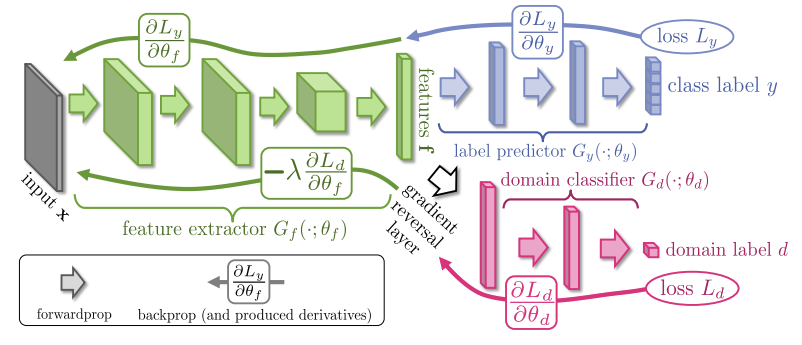
\includegraphics[width=0.48\linewidth]{figures/related_work/DANN.png}%
    }\hfill
    \subfigure[SHOT机制~\cite{liang2021source}]{%
    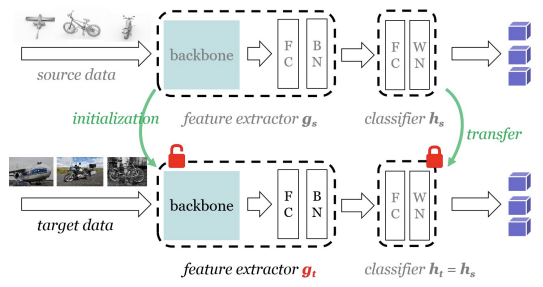
\includegraphics[width=0.48\linewidth]{figures/related_work/SHOT.png}%
    }
    \bicaption[fig:da_works]{}{域迁移代表方法}{Fig.}{Representative methods for domain adaptations}
\end{figure}

在 UDA 方法谱系之上，进一步收紧至“源数据不可访问”这一严格设定，即得到无源域适应（Source-Free Domain Adaptation, SFDA）~\cite{liang2021source}。该设定下，原有方法所依赖的源数据统计量、域判别信号、跨域重构样本与伪标签生成机制均无法直接调用，必须在仅有源模型参数的条件下构造新的跨域监督。源假设迁移（Source-Hypothesis Transfer, SHOT）~\cite{liang2021source} 通过冻结源分类器对目标特征聚类生成伪标签，成为该方向的开创性工作；NRC~\cite{yang2021neighbor} 利用邻居关系约束类内一致性；CoWA-JMDS~\cite{cowa}、U-SFAN~\cite{U-SFAN} 引入模型不确定性或数据不确定性估计对伪标签进行加权；D-MCD~\cite{chu2022denoised} 通过双分类器对抗训练识别高置信度样本中的噪声；VDM-DA~\cite{tian2022vdm} 借助虚拟域判别器选择熵值较低的干净伪标签；SSNLL~\cite{chen2022self} 以指数滑动平均模型对样本进行分层处理；Kundu 等人~\cite{kundu2022towards} 进一步从信息瓶颈角度给出 SFDA 目标风险的显式上界，为上述方法提供理论解释。综合而言，SFDA 在 UDA 方法谱系之上，叠加了以伪标签驱动、邻域约束与不确定性估计为核心的样本级跨域不变性学习机制，构成了无监督模型迁移域不变学习方法范式维度下的第一条技术主线。


方法范式决定了跨域监督信号的构造方式，骨干架构则决定了跨域不变特征在底层表征空间中的捕获能力，两者协同决定最终的迁移效果。骨干网络的设计深刻影响实例级跨域不变特征的捕获能力，呈现出从 CNN 局部感受野到 ViT 全局注意力、再到选择性扫描状态空间模型（State-Space Model, SSM）Mamba 线性长程建模的清晰演进脉络。CNN（尤其是 ResNet~\cite{he2016deep}）凭借层次化特征聚合的归纳偏置~\cite{yang2021neighbor,xia2021adaptive,zhang2024nami}，是大量域迁移的默认选择；然而固定局部感受野难以捕获跨区域对象结构关系~\cite{long2015learning,ganin2016domain}。针对这一局限，ViT~\cite{dosovitskiy2021image} 通过自注意力机制实现全局感受野~\cite{sanyal2023stable,xia2024dual}，DSIT~\cite{sanyal2023dsit}、TransDA~\cite{TransDA}、C-SFTrans~\cite{sanyal2024aligning}、DPC~\cite{dpc} 等工作将 ViT 引入域适应；但 $\mathcal{O}(N^2)$ 的注意力复杂度在高分辨率图像上带来难以承受的计算开销~\cite{zhu2024vision}。作为替代，Vim~\cite{zhu2024vision}、VMamba~\cite{vmamba} 将 Mamba 扩展到视觉建模，通过双向与四向扫描策略以线性复杂度实现全局感受野~\cite{zhu2024vision,vmamba}。在域适应场景下，DA-Mamba~\cite{DA-Mamba} 进一步将 Mamba 引入跨域目标检测任务，缓解 CNN 的全局语义忽略与 ViT 的高计算开销。综合而言，沿骨干架构从 CNN 到 ViT 再到 SSM 的演进路径，系统探索跨域不变特征的捕获机制，构成无监督模型迁移域不变学习骨干架构维度下的第二条技术主线。

\subparagraph{少监督域适应方法}

当源—目标域差异较大时，仅靠全无标注的自学习路径难以进一步压缩目标域误差，一种自然思路是在迁移过程中引入少量人工标注以提升监督信号的可靠性，由此衍生出少监督域适应方法。从标注样本的来源与源域可见性两个维度刻画，少监督域适应方法可划分为四种典型设定：标注样本由训练集预先给定的半监督域适应（Semi-Supervised Domain Adaptation, SSDA）及其在极低监督下的极端收紧形态——少样本域适应（Few-Shot Domain Adaptation, FSDA），对应源域可访问、标注预算固定分配的常见场景；标注样本由模型在无标注目标域池中主动筛选的主动域适应（Active Domain Adaptation, ADA），对应源域可访问、标注预算由模型主导分配的场景；以及在上述任一形式上进一步收紧至“源数据不可访问”假设的主动无源域适应（Source-Free Active Domain Adaptation, SFADA）。SSDA/FSDA 与 ADA 在标注来源维度上互补，SSDA/FSDA/ADA 与 SFADA 在源域可见性维度上递进收紧，共同构成少监督域适应方法的两条正交设计维度。

\begin{figure}[!htbp]
    \centering  
    \setlength{\tabcolsep}{0pt}
    \subfigure[MME学习框架~\cite{saito2019semi}]{
        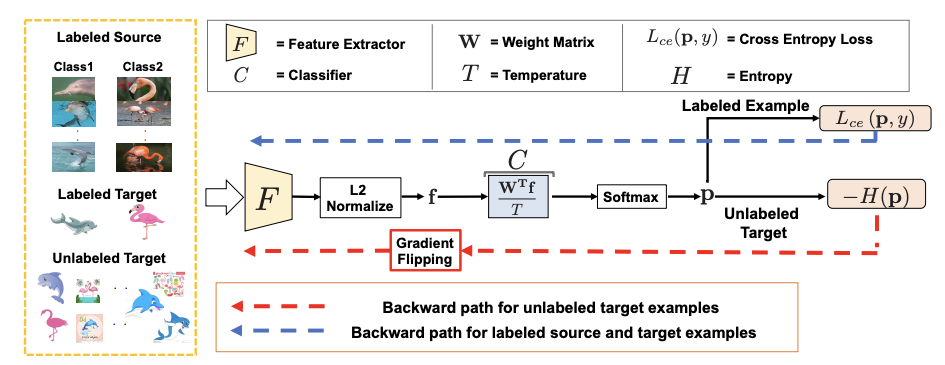
\includegraphics[width=0.48\linewidth]{figures/related_work/MME.png}
    }\hfill
    \subfigure[MHPL样本选择~\cite{MHPL}]{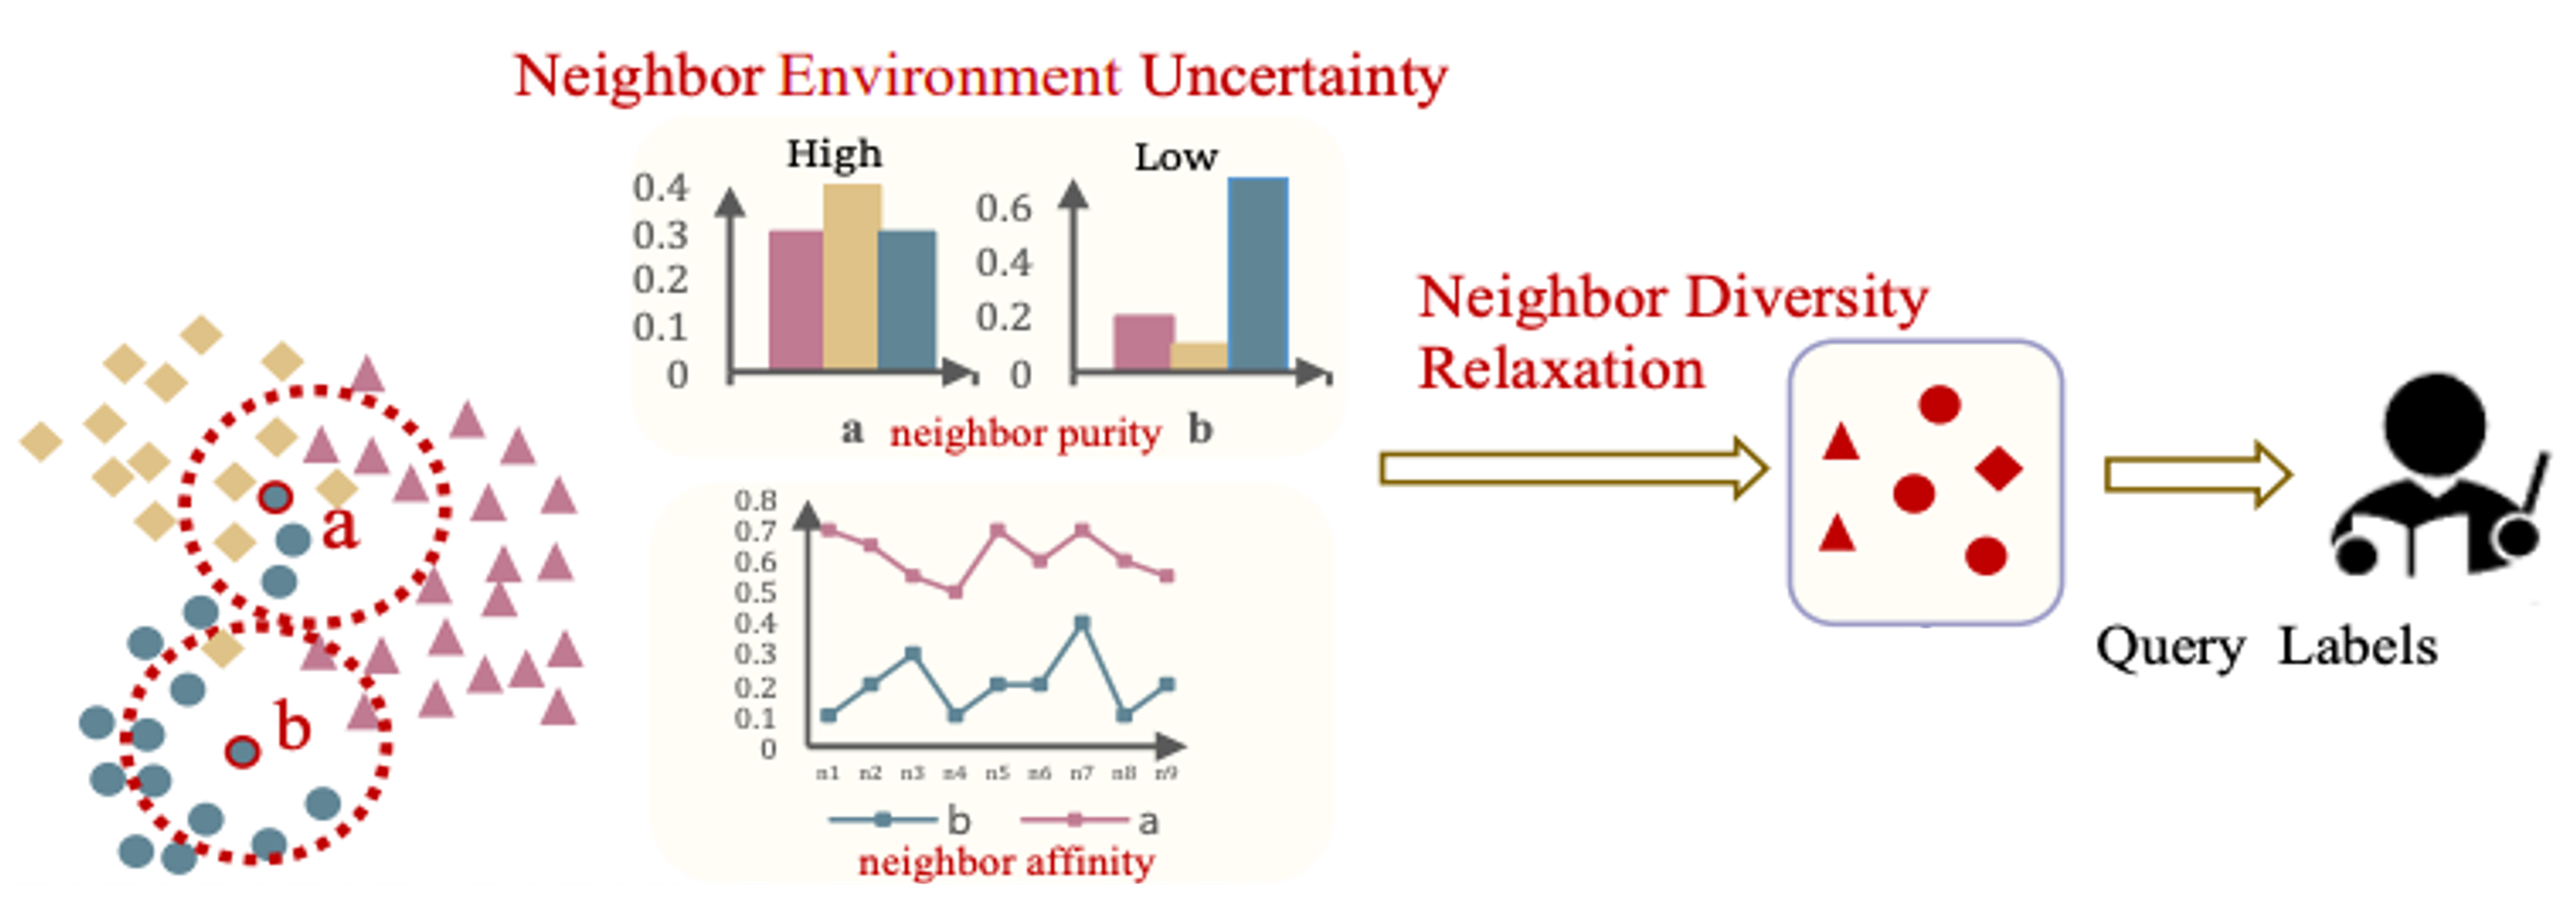
\includegraphics[width=0.48\linewidth]{figures/related_work/MHPL.png}}
    \bicaption[fig:rare_da]{}{少监督域适应代表方法}{Fig.}{Representative methods for limited-supervision domain adaptation}
\end{figure}

半监督与少样本域适应设定了有限标注目标样本（每类 1 至 N 个）+ 大量无标注目标样本的标准少监督范式，是少监督域适应方法谱系中最一般化的形式。SSDA 的开创性工作 MME~\cite{saito2019semi} 通过对抗式最小化最大熵同时利用标注与无标注目标样本的边缘分布；后续工作进一步围绕伪标签去噪、对比约束与一致性正则等机制扩展 SSDA 设定下的跨域监督构造。FSDA 进一步收紧至每类仅 1–5 个标注目标样本的极端设定，借助度量学习、元学习或跨域原型对齐缓解极低监督下的过拟合问题~\cite{zhao2021fewshot}。SSDA/FSDA 与 UDA 共同构成了域适应方法谱系中“源域可访问、目标域可借助少量人工标注”的最一般形式。

将主动学习策略与域适应结合，即形成主动域适应（Active Domain Adaptation, ADA）。在通用机器学习场景下，主动学习是应对有限标注预算的经典策略，其核心假设是并非所有未标注样本对模型改善的贡献相同，应优先选择对监督信号贡献最大的样本加以标注。具体而言，不确定性采样选择预测高熵的样本以最大化单次标注的信息增益，代表性采样则通过 CoreSet~\cite{CoreSet1} 求解 K-Center 贪心问题使所选子集覆盖全部样本的几何结构；二者从不同维度互补，构成了主动学习的两种核心路径。Mathelin 等人~\cite{mathelin2022discrepancy} 进一步从理论角度区分模型不确定性（可通过更多数据降低）与数据不确定性（由输入固有噪声决定），为上述两种采样策略提供了可解释的概率基础。在 ADA 设定下，CLUE~\cite{prabhu2021active}、EADA~\cite{xie2022active}、CA-ADA~\cite{xiao2024category} 等代表性工作将上述样本选择机制与域偏移度量结合，使所选标注样本同时具备对当前模型的不确定性与对目标域分布的代表性。
进一步收紧至“源数据不可访问”这一严格设定，ADA 衍生为主动无源域适应（Source-Free Active Domain Adaptation, SFADA），其核心挑战是源数据不可用带来的伪标签噪声放大与外部监督信号缺失。MHPL~\cite{MHPL} 通过联合邻居一致性、个体差异性与域差异性进行样本筛选；ELPT~\cite{li2022source} 优先选择局部结构尚不清晰的样本；SQAdapt~\cite{SQAdapt} 借助数据增强下的预测敏感性度量样本价值；Wang 等人~\cite{wang2023mhpl} 与 Li 等人~\cite{li2023source} 对 SFADA 的设定与挑战给出系统性总结。

视觉—语言基础模型（Vision-Language, ViL）在少监督域适应的跨模型监督中也发挥重要作用。CLIP~\cite{radford2021learning} 与 ALIGN~\cite{jia2021scaling} 凭借海量图文对比学习建立了视觉—语义统一嵌入空间，具备出色的零样本泛化能力；其下游适配策略主要分为三类——提示学习（CoOp~\cite{zhou2022learning}、KgCoOp~\cite{kgcoop}）、参数高效适配器（Tip-Adapter~\cite{Tip-Adapter}）、以及伪标签微调方法（PADCLIP~\cite{lai2023padclip}）。在 UDA 设定下，DAPL~\cite{ge2023domain} 将上下文分解为域无关与域相关部分以解耦语义与域偏置，PADCLIP~\cite{lai2023padclip} 通过调整学习率缓解 CLIP 微调中的灾难性遗忘；在 SFDA 设定下，DIFO~\cite{tang2024source} 通过最大化目标模型与 CLIP 之间的互信息，将 CLIP 的零样本语义知识蒸馏到目标模型。然而现有方法在将 ViL 与目标模型结合时多停留于浅层组合，缺乏理论指导下的双向深度交互机制。

综上，面向样本实例的跨域不变特征学习指向一个核心问题：如何在方法范与骨干架构两条正交维度上协同突破，使模型在“无标注”与“少量标注”两种极端设定下均能实现可靠的跨域不变特征学习。

\subsection{面向类别概念的跨域语义关系学习}

开放类别识别是视觉感知的核心需求之一。传统有监督学习在封闭类别 设定下依赖大规模标注数据训练特定分类器，难以扩展至训练时未见 的新类别；跨域语义关系学习旨在突破这一限制——通过挖掘类别 概念之间的语义关联（属性、文本描述、视觉—语言嵌入等侧信息）， 构建对未见类别与新词表具备泛化能力的视觉识别系统。

% 本节按照 从"域偏移下的开类识别"到"开放词表开放世界开类学习"的 递进关系展开：先回顾在域偏移设定下借助语义侧信息识别未知类的 开集域适应与广义零样本工作；进而讨论在无类别边界约束的开放 词表下，利用视觉—语言基础模型与分割基础模型实现像素级开放 词汇分割的最新进展；最后归纳当前研究在统一解码框架深度融合 方面的不足，引出本论文第 4 章的切入角度。

\subparagraph{域偏移下的开类识别}

开集域适应（Open-Set Domain Adaptation, OSDA）将传统域适应从“已见类跨域对齐”扩展到“在跨域迁移中同时识别未知类”，是域偏移下开类识别的代表性设定。与封闭集域适应相比，OSDA 不再假设源—目标域共享同一封闭类别空间，而是承认目标域中可能出现训练时未标注的未知类别，因此要求模型在完成跨域特征对齐的同时，赋予未知类样本独立的“未知”占位判别能力。这一设定广泛存在于工业缺陷检测、医学病灶诊断等真实场景——目标域类别数往往无法被源域类别集完全覆盖。

围绕如何在保留域不变特征的同时刻画未知类，OSDA 衍生出多条技术路线。分离式方法~\cite{liu2021separate} 通过渐进式分离将已知类与未知类样本在特征空间内逐步拉开距离；继承式方法~\cite{kundu2022towards} 提出可继承的源模型结构，使源分类器在目标域未知类新增时仍能保持已见类的判别能力；校正式方法~\cite{li2023adjustment} 引入未知类偏置校正，补偿分类器对未知类样本的判别阈值漂移；关系式方法~\cite{tong2025reserve} 通过挖掘类间语义关系在共享类与未知类之间建立桥梁，利用属性或文本侧信息辅助未知类定位；多域扩展方面，~\cite{liu2025open} 将 OSDA 推广至混合域场景，借助视觉—语言聚焦机制同时应对多个目标域的开放识别需求。在无源数据设定下，~\cite{wang2025active} 将 OSDA 与主动学习结合，在源数据不可访问的严格约束下通过少量人工标注主动识别未知类。

与广义零样本学习（Generalized Zero-Shot Learning, GZSL）相比，OSDA 的核心差异在于对未知类的“可见性”假设——GZSL 假设测试阶段可见到所有未见类样本但无对应训练样本，OSDA 则仅假设目标域中含有未知类且不提供任何先验语义信息，因此两者的技术挑战与解决路径存在本质差异。但二者共同体现了“在跨域或跨类别的开放设定下进行识别”这一核心问题。

整体而言，OSDA 工作的核心假设仍是“未知类不可见、但目标域一定含有未知类”，仍依赖于“已知类标签 + 未知类占位”的双分支判别结构，对类别语义侧信息的利用也以已知类内部的语义关联为主，尚未真正引入“任意自然语言描述作为类别”的开放词表机制。这一局限为开放词表识别方向的兴起埋下伏笔。

\subparagraph{开放世界开类学习}

随着视觉—语言基础模型在零样本分类、跨模态检索等任务上 展现出强大的开放语义能力，研究焦点从“有限未知类的开集 识别”推进到“无类别边界约束的开放词表识别（Open-Vocabulary Recognition, OVR）”——即在测试阶段面对任意自然语言描述的 新类别时仍能完成识别。这一开放词表识别能力在检测与分割 两个密集预测任务上分别衍生出开放词汇检测（Open-Vocabulary Detection, OVD）与开放词汇分割（Open-Vocabulary Segmentation, OVS）~\cite{liu2026open}。OVS 要求模型在训练时未见过的新类别上仍能完成像素级 识别与分割，其难度集中体现为两类基础模型能力的耦合：一类是分割基础模型（Segment Anything Model, SAM）~\cite{kirillov2023segment}所提供的像素级 空间定位能力，另一类是 CLIP~\cite{radford2021learning}、 ALIGN~\cite{jia2021scaling} 等视觉—语言基础模型所提供的开放 词汇语义理解能力。然而两类先验长期独立演进，如何在统一 解码框架内深度融合二者，成为该方向亟需回应的核心问题。

\begin{figure}[!htbp]
    \centering  
    \setlength{\tabcolsep}{0pt}
    \subfigure[两阶段方法OVSeg框架图~\cite{liang2023open}]{
        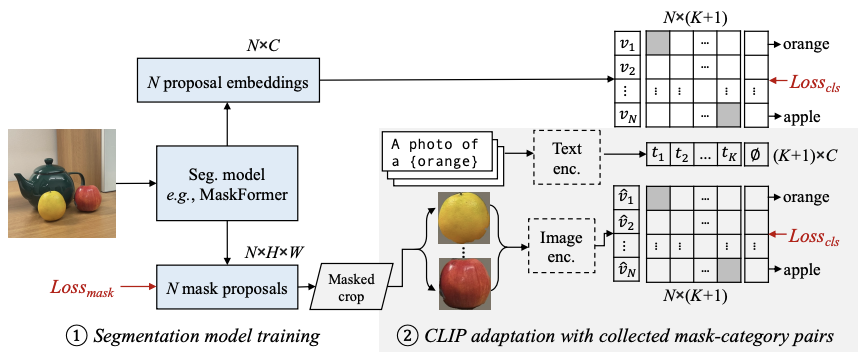
\includegraphics[width=0.48\linewidth]{figures/related_work/ovseg.png}
    }\hfill
    \subfigure[单阶段方法FC-CLIP框架图~\cite{yu2023convolutions}]{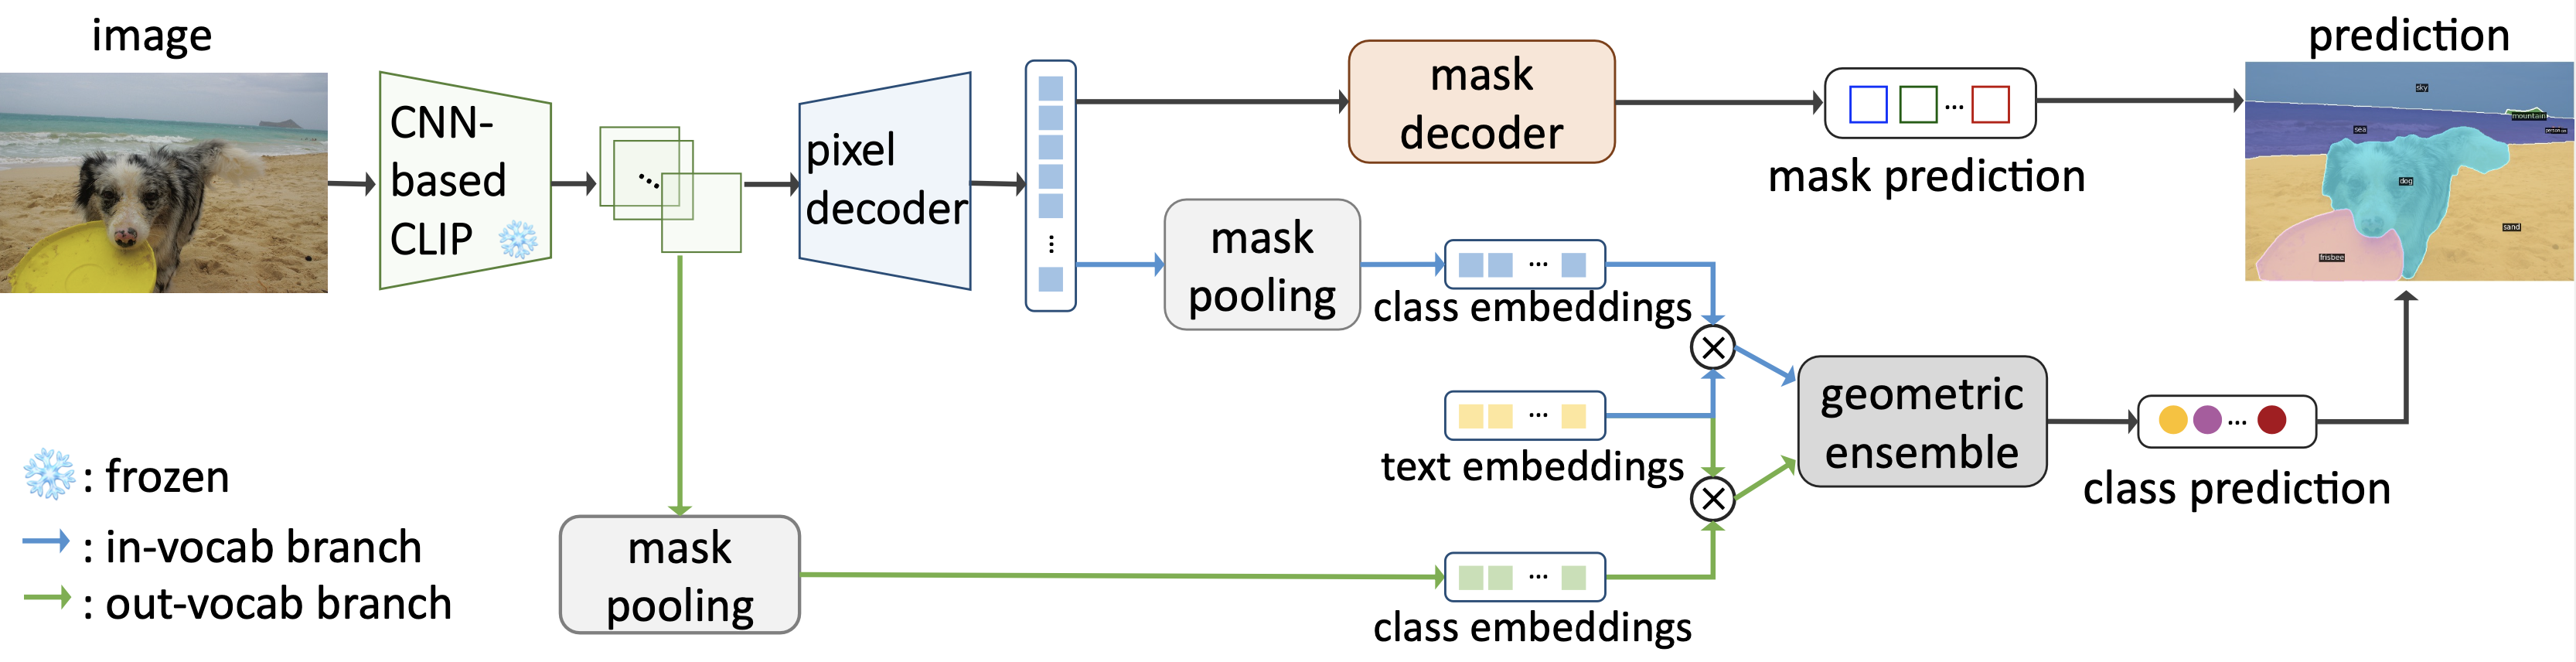
\includegraphics[width=0.48\linewidth]{figures/related_work/fc-clip.png}}
    \bicaption[fig:rare_ovs]{}{代表的开放词表方法}{Fig.}{Representative methods for open-vocabulary methods}
\end{figure}

OVS 方法可沿“先生成掩码再分类”的两阶段路径与“端到端 单阶段”两条主线展开。两阶段方法~\cite{liu2024open,maskclip,xu2022simple,MasQCLIP,liang2023open,chen2023open} 一般先借助额外分割模型生成类别无关掩码提议，再将 ViL 特征与多个掩码提议进行交互以分配语义类别。SCAN~\cite{liu2024open} 通过双流网络联合学习语义无关的掩码与类别嵌入；MaskCLIP~\cite{maskclip} 以类别无关掩码与可学习 mask token 与 CLIP 嵌入交互；OPSNet~\cite{chen2023open} 将 mask query 嵌入与 CLIP 最后一层嵌入结合用于域外类别识别， 并引入 IoU 分支过滤低质量提议；OVSeg~\cite{liang2023open} 通过在大规模开放词汇数据上微调掩码分类器提升密集预测 质量；SimBase~\cite{xu2022simple} 与 MasQCLIP~\cite{MasQCLIP} 进一步简化两阶段流水线并探索 CLIP patch 特征与掩码的对齐。 两阶段方法的主要局限是“先生成、再分类”的串行结构导致 特征不对齐与计算冗余，且对未见类别的掩码质量高度依赖 上游提议模型。

单阶段方法~\cite{yu2023convolutions,wu2024clipself,MGCCL} 将 ViL 模型本身扩展为分割器骨干，端到端地完成密集预测，避免了 掩码提议阶段带来的过拟合风险。FC-CLIP~\cite{yu2023convolutions} 通过在 CLIP 之上引入掩码分类头实现单阶段开放词汇分割； CLIPSelf~\cite{wu2024clipself} 在 CLIP 内部通过自蒸馏提升 patch 级别表征；MGCCL~\cite{MGCCL} 借助多粒度对比学习增强 文本—图像—掩码三方的语义对齐。研究表明，卷积式 CLIP 模型相较 ViT 式 CLIP~\cite{dosovitskiy2021image} 在大输入 分辨率下表现更优，这与其对空间结构的局部归纳偏置密切相关。 然而，CLIP 的 patch 级特征本质上是为图像级识别设计的， 缺乏细粒度的像素级监督，因而在 mask 边界精度与对小目标 的捕捉上存在天然上限。

视觉—语言基础模型与分割基础模型的融合是 OVS 突破上述 瓶颈的关键路径。CLIP 与 ALIGN 在零样本分类、检索、跨模态 匹配等任务上展现强大泛化能力；SAM 凭借十亿级分割掩码 训练实现任意提示引导的零样本实例分割。SAM 的适应性通过 多种提示策略进一步增强，包括低级视觉提示~\cite{MMRAD}、 弱监督~\cite{ROSE} 等；同期工作 SEEM~\cite{seem} 将空间 提示（点、框、涂鸦、掩码）与文本提示统一到联合图像—文本 表征空间；X-Decoder~\cite{zou2023seg} 通过不同 query 类型 实现任务统一。然而 SAM 本身不输出类别语义，CLIP 又缺乏 像素级密集监督，二者在统一解码框架内的深度融合仍有待 探索。RegionSpot~\cite{yang2024recognize} 通过开放词汇 检测器生成候选框并送入 SAM 完成高质量分割；Open-Vocabulary SAM~\cite{yuan2024open} 借助交互式提示在二十千类上完成 分割与识别。然而上述方法多以“检测器 + SAM”或“CLIP + 分割器” 的松耦合方式组合，掩码质量与类别语义识别之间仍存在错配： SAM 的高质量掩码与 CLIP 的开放语义难以在统一解码框架内 对齐。从松耦合到紧耦合的范式演进中，基础模型融合范式 经历了从外部检测器 + 分割器的两阶段流水线到单阶段 CLIP 骨干 + 分割头的端到端融合、再到跨模型统一解码 的演进。

但 CLIP 本身的 patch 级特征存在三方面局限：1. patch 间 存在显著的区域级偏置，对象边界与 patch 网格不对齐； 2. 图像—文本对比的训练目标缺少像素级监督，对小目标 与精细结构的刻画不足；3. 推理阶段文本—视觉相似度的 计算开销与类别数线性相关，开放词汇场景下需配合高效的 类别嵌入压缩。现有缓解思路包括 FC-CLIP~\cite{yu2023convolutions} 通过卷积 CLIP 提升分辨率适应性、DenseCLIP~\cite{rao2022denseclip} 引入像素—文本密集对齐、CLIPSelf~\cite{wu2024clipself} 通过自蒸馏提升 patch 级表征、MGCCL~\cite{MGCCL} 借助 多粒度对比学习联合优化。
% 然而上述方法均未在统一解码 框架内充分利用 SAM 的高质量掩码先验，导致掩码质量与 语义识别之间的错配。


\subsection{面向高层语义的理解范式构建}

多模态大语言模型（Multimodal Large Language Model, MLLM）的兴起重新定义了视觉语义理解的层次边界。与传统视觉模型相比，MLLM 将视觉感知与语言推理统一到语言模型的推理框架之下，使其不仅具备图像级识别能力，更能够进行开放词汇推理、跨模态常识推理与高阶语义抽取，形成从“感知层”到“概念层”再到“综合推理层”的语义理解层次跨越。围绕 MLLM 的语义理解能力，现有关键工作沿感知层、概念层与综合推理层三个层次展开，艺术情感理解作为“感知—认知—情感”深度交织的高阶语义推理任务，是检验 MLLM 跨层语义理解能力的典型综合测试平台。
% 本节梳理 MLLM 在感知层语义理解、概念层语义理解与艺术情感综合推理三个层面的相关工作，为第 5 章面向艺术情感推理的多层级评测基准研究提供背景铺垫。

上一节聚焦于“跨域迁移”语境下的类别语义学习；本节将研究视野从“跨域”拓展至“跨层”，关注 MLLM 在感知层的像素级定位与基本属性识别、概念层的抽象推理与知识迁移，与综合推理层的感知证据与情感归因的协同推理上的能力边界与评测方法。


感知层语义理解是 MLLM 跨层语义推理的基础。MLLM 在视觉定位、属性识别与空间关系推理等感知任务上取得了显著进展，代表性开源模型包括 LLaVA~\cite{liu2023llava_neurips}、MiniGPT-4~\cite{zhu2024minigpt4}、Shikra~\cite{shikra2023referential} 等。这些模型均以 CLIP 系列视觉编码器建立视觉—语言对齐，在感知层面超越传统视觉模型；在此基础上，开放词汇感知能力进一步通过工业级模型 Gemini~\cite{comanici2025gemini} 得到验证。感知层评测方面，MMBench~\cite{mmbench2023}、SeedBench~\cite{seedbench2024} 等选择题基准与 GAVIE~\cite{liu2024gavie} 等 GPT-4 辅助开放式评分方法均表明，现有感知层评测维度较为单一，难以诊断模型在复杂感知场景（如小目标检测、遮挡推理、跨视角一致性）下的真实能力边界。


\begin{figure}[!htbp]
    \centering  
    \setlength{\tabcolsep}{0pt}
    \subfigure[视觉-语言模型多模态能力评测基准MMBench~\cite{mmbench2023}]{
        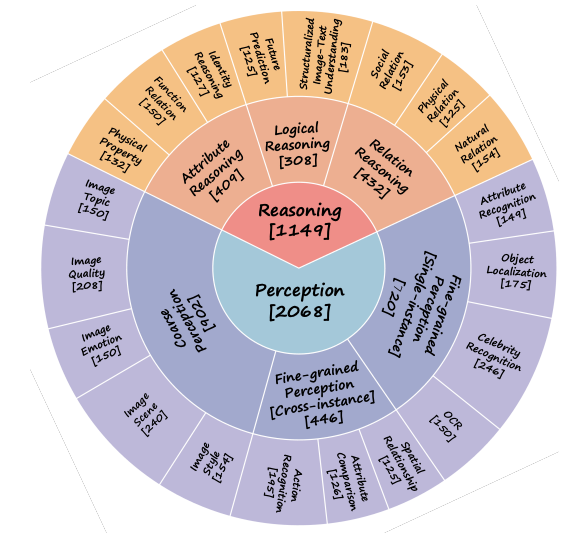
\includegraphics[width=0.48\linewidth]{figures/related_work/mmbench.png}
    }\hfill
    \subfigure[图像情感评测基准EEmo-Bench~\cite{eemobench2025}]{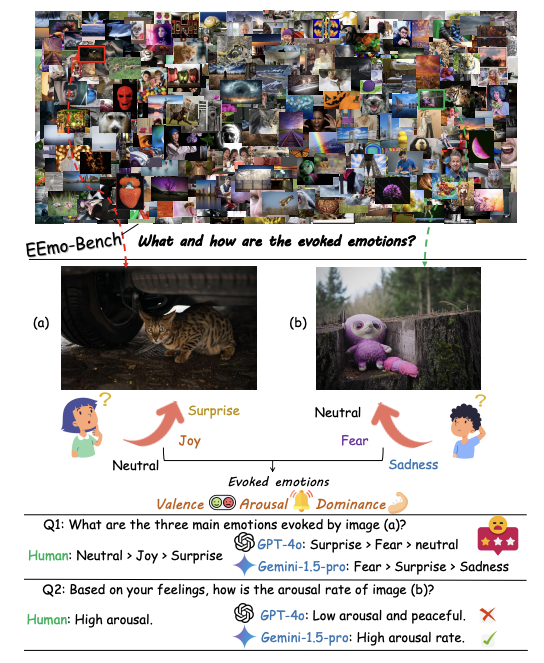
\includegraphics[width=0.38\linewidth]{figures/related_work/EEmo-Bench.png}}
    \bicaption[fig:related_benchmarks]{}{代表性的语义评测基准}{Fig.}{Representative benchmarks for semantic evaluation}
\end{figure}

概念层语义理解超越了“图像中有什么”的感知范畴，要求模型在抽象概念、因果推理与跨模态知识迁移等层面进行高阶推理。ScienceQA~\cite{lu2022scienceqa}、MMMU~\cite{yue2024mmmu} 等基准揭示了 MLLM 在科学推理与多学科知识问答上的潜力，也暴露了其“幻觉”与推理链断裂等问题。具体到视觉领域，概念层理解体现在“构图风格”“情感隐喻”“文化符号”等抽象视觉语义的识别能力上——这恰是艺术情感推理区别于普通图像理解的核心所在。情感维度理论~\cite{yang2023emoset,you2016building} 将连续情感空间映射到VAD-Valence（效价）、Arousal（唤醒度）、Dominance（支配度）三维度，弥补了离散情感标签粒度不足的问题，但当前 MLLM 对 VAD 三维度的估计能力尚未得到系统性诊断。

艺术情感综合推理是检验 MLLM 跨层语义理解能力的典型测试平台。艺术图像的情感表达往往隐含在构图、笔触、风格化与文化符号之中，而非由具体对象或事件显式承载，这使得传统以低层视觉描述子或离散情感标签为主线的情感计算方法在艺术场景下面临显著局限。进入 MLLM 时代后，ArtEmis~\cite{achlioptas2021artemis} 收集了艺术作品的情感反应与解释，揭示了艺术欣赏中“主观但视觉有据”的语言特征；EEmo-Bench~\cite{eemobench2025} 引入 VAD 多维情感描述与配对图像比较；EmoSet~\cite{yang2023emoset} 强调视觉证据在情感理解中的重要性。然而现有基准普遍未系统拆分感知、情感归因、基于证据的推理与开放式描述四个认知子维度，评测结论因而停留在事实正确性或表述流畅度这类单一维度上，无法把流畅措辞与可靠解释置于同一证据标尺下加以判定——这正是当前 MLLM 艺术情感评测的核心缺口。

综上，MLLM 跨层语义理解评测当前面临的核心瓶颈是缺少面向高阶语义推理的诊断型评测协议：现有基准多以选择题或简短问答形式评测感知层与概念层能力，对综合推理层（如“感知—情感—推理—描述”四个认知层次的协同诊断）覆盖不足，难以将“流畅的情感表述”与“基于视觉证据的可靠解释”区分开来。

\subsection{现有方法的主要问题}

\noindent\textbf{（1）现有无监督方法在跨域分布偏移下的不确定性建模与表征鲁棒性上存在瓶颈}

跨数据域分布偏移是模型迁移研究中的核心挑战：当目标域与源域分布存在显著差异，如何获得可靠的跨域不变监督信号并学习对域偏移鲁棒的表征，是模型迁移设定下的基本研究问题。现有方法在不确定性估计与表征鲁棒建模两个层面均存在不足：在不确定性估计层面，伪标签去噪多依赖经验式筛选准则，缺乏可量化的样本级不确定性估计机制，难以稳定区分跨域预测的可靠程度；在表征鲁棒建模层面，沿不同骨干路径展开的现有方法难以在长程依赖建模、计算效率与空间语义对齐之间取得有效平衡，且多假设源数据可访问，缺乏对模型迁移设定下骨干结构选型与不确定性传播抑制的协同设计。因此，如何在跨数据域分布偏移下协同突破不确定性估计与表征鲁棒建模两个层面，是模型迁移研究亟待解决的核心问题。

\noindent\textbf{（2）现有少监督方法在信息驱动的样本挖掘与跨模态协同上存在不足}

在目标域仅有少量标注样本可用的稀缺监督条件下，如何拓展监督信号的来源与协同深度，是模型迁移设定下的另一关键研究问题。视觉—语言等大模型凭借大规模跨模态预训练获得了对开放语义的零样本判别能力，其预测不依赖源域分布，能够为目标样本提供与源模型假设空间互补的语义判断信号，这对缓解源模型在目标域上的预测偏置、扩展稀缺标注预算下的监督信息量具有重要价值。然而现有方法在样本选择与跨模型协同两个环节均缺乏对多模态预训练模型监督信号的系统探索，未能建立视觉—语言模型与源模型在信息驱动采样与双向深度协同层面的严谨理论框架。因此，如何实现视觉—语言模型与源模型在信息驱动采样与双向深度协同层面的协同，是模型迁移研究需要解决的关键问题。

\noindent\textbf{（3）现有跨类泛化方法在多流语义对齐与空间定位上探索不足}

视觉—语言模型与分割基础模型分别提供了开放词表的语义锚点与像素级空间定位能力，二者的协同融合被视为突破该问题的关键路径。然而现有方法在多流语义对齐与空间定位两个层面均存在不足：在多流语义对齐层面，两阶段与单阶段方案均难以在统一框架下实现掩码生成与开放词汇识别之间的深度协同；在空间定位层面，现有方案难以同时兼顾对像素级对齐的精细建模与对未见类别的掩码质量，致使对长尾与未见类别的细粒度识别能力受限。因此，如何在统一解码框架内深度融合分割基础模型的空间定位能力与视觉—语言模型的开放词汇语义能力，通过多流语义对齐与空间定位的协同优化实现对长尾与未见类别的泛化，是跨类泛化研究亟待解决的核心问题。

\noindent\textbf{（4）现有语义理解标准在证据锚定与评测维度建模上存在缺口}

语义理解要求模型在开放式语义理解的基础上具备对抽象语义与文化背景的稳健推理能力。语义类评测相对事实类评测具有显著的特殊性：受主观性、抽象性与文化语境三重影响，语义类内容的可靠解释难以被“事实正确性”或“流畅表述”等单一维度度量，这使得传统以事实判断或选择题为主的评测标准在语义理解评测上存在结构性局限。在证据锚定层面，现有方法未能将语义归因与视觉证据进行细粒度绑定；在评测维度建模层面，现有语义评测多沿用单维分类或简短问答形式，未能系统拆解互补的认知子维度。因此，如何构建兼具结构化诊断能力与开放式评分灵活性的多层级多维度评测标准，是语义理解标准研究亟待突破的核心方向。

\section{本文的主要研究内容及组织结构}

\subsection{本文的研究内容}

从前文分析可以看出，模型迁移研究在多种泛化场景下面临根本性挑战。与常规同分布训练不同，泛化场景要求模型在数据分布、词表覆盖或语义层级与训练阶段存在差异的条件下保持稳定性能，且源域数据往往不可访问或仅有少量标注可利用。这一约束使传统的“训练—测试同分布”假设被打破，模型需要从有限的目标侧信息与多模态预训练先验中提取可迁移知识，构成本文区别于普通图像理解的核心研究问题。围绕这一核心问题，本文从域泛化、类泛化、语义理解泛化三个层面展开研究。具体围绕下面四个关键问题展开。


\noindent\textbf{（1）无监督模型迁移的不确定性抑制问题}

域分布偏移下，伪标签去噪缺乏可量化的样本级不确定性估计机制，骨干结构对跨域不确定性的传播方式对表征鲁棒性具有决定性影响。本文从不确定性源头抑制与传播路径阻断两个层面协同突破：在源头层面，挖掘特征空间的样本级结构信息以量化伪标签层的不确定性，避免引入额外模型带来的偏差与代价；在传播层面，抑制虚假相关性在跨通道与跨空间维度上的累积放大，从源头与扩散两个层面共同提升模型迁移的可靠性。

\noindent\textbf{（2）少监督模型迁移的信息最大化问题}

稀缺监督条件下，视觉—语言模型的开放语义先验能够为目标样本提供与源模型假设空间互补的语义判断信号，但现有方法在跨模型协同上未能将视觉—语言模型作为协同监督信号进行理论严谨的双向深度协同。本文从理论建模与跨模态协同两个层面突破：在理论层面，推导主动无源域适应设定下稀缺标注与开放语义先验协同监督的风险上界；在协同机制层面，构建视觉—语言模型与目标模型的双向深度协同框架，使两类互补信号在样本空间与假设空间两个层面实现增量互补。

\noindent\textbf{（3）模型泛化的多模态类别先验挖掘问题}

跨类泛化的核心要求是模型对训练阶段未见过的新颖类别保持识别能力，其关键在于系统挖掘并融合多源类别先验。现有方法多沿单一先验源或粗粒度拼接展开，缺乏在不同网络层级上的双向注入与协同机制。本文从多层级协同融合与双向耦合两个维度展开：在多层级协同融合层面，使空间定位与开放词汇语义两类先验在不同网络深度上交叉作用而非简单串接；在双向耦合层面，使两类先验在网络前向推理中相互增强而非单向辅助，从而在多个细粒度识别任务上取得优于现有方法的性能。

\noindent\textbf{（4）多维度语义理解标准制定问题}

语义理解评测标准在证据锚定与评测维度建模上存在结构性缺口，传统以事实判断或选择题为主的评测标准难以度量语义类内容的可靠解释；现有方法未能将语义归因与视觉证据进行细粒度绑定；评测维度建模多沿用单维分类或简短问答形式，未能系统拆解多个认知子维度。本文围绕证据化解释与多维度诊断两个核心要素展开：在证据化解释层面，使基于视觉证据的可靠解释与缺乏视觉依据的语义表述成为可被精准区分的评测对象；在多维度诊断层面，将语义理解能力沿互补认知层级拆解并设计兼顾结构化诊断与开放式评分的综合评测协议。

\subsection{本文的组织结构}

\begin{figure}[!htbp]
 \centering
 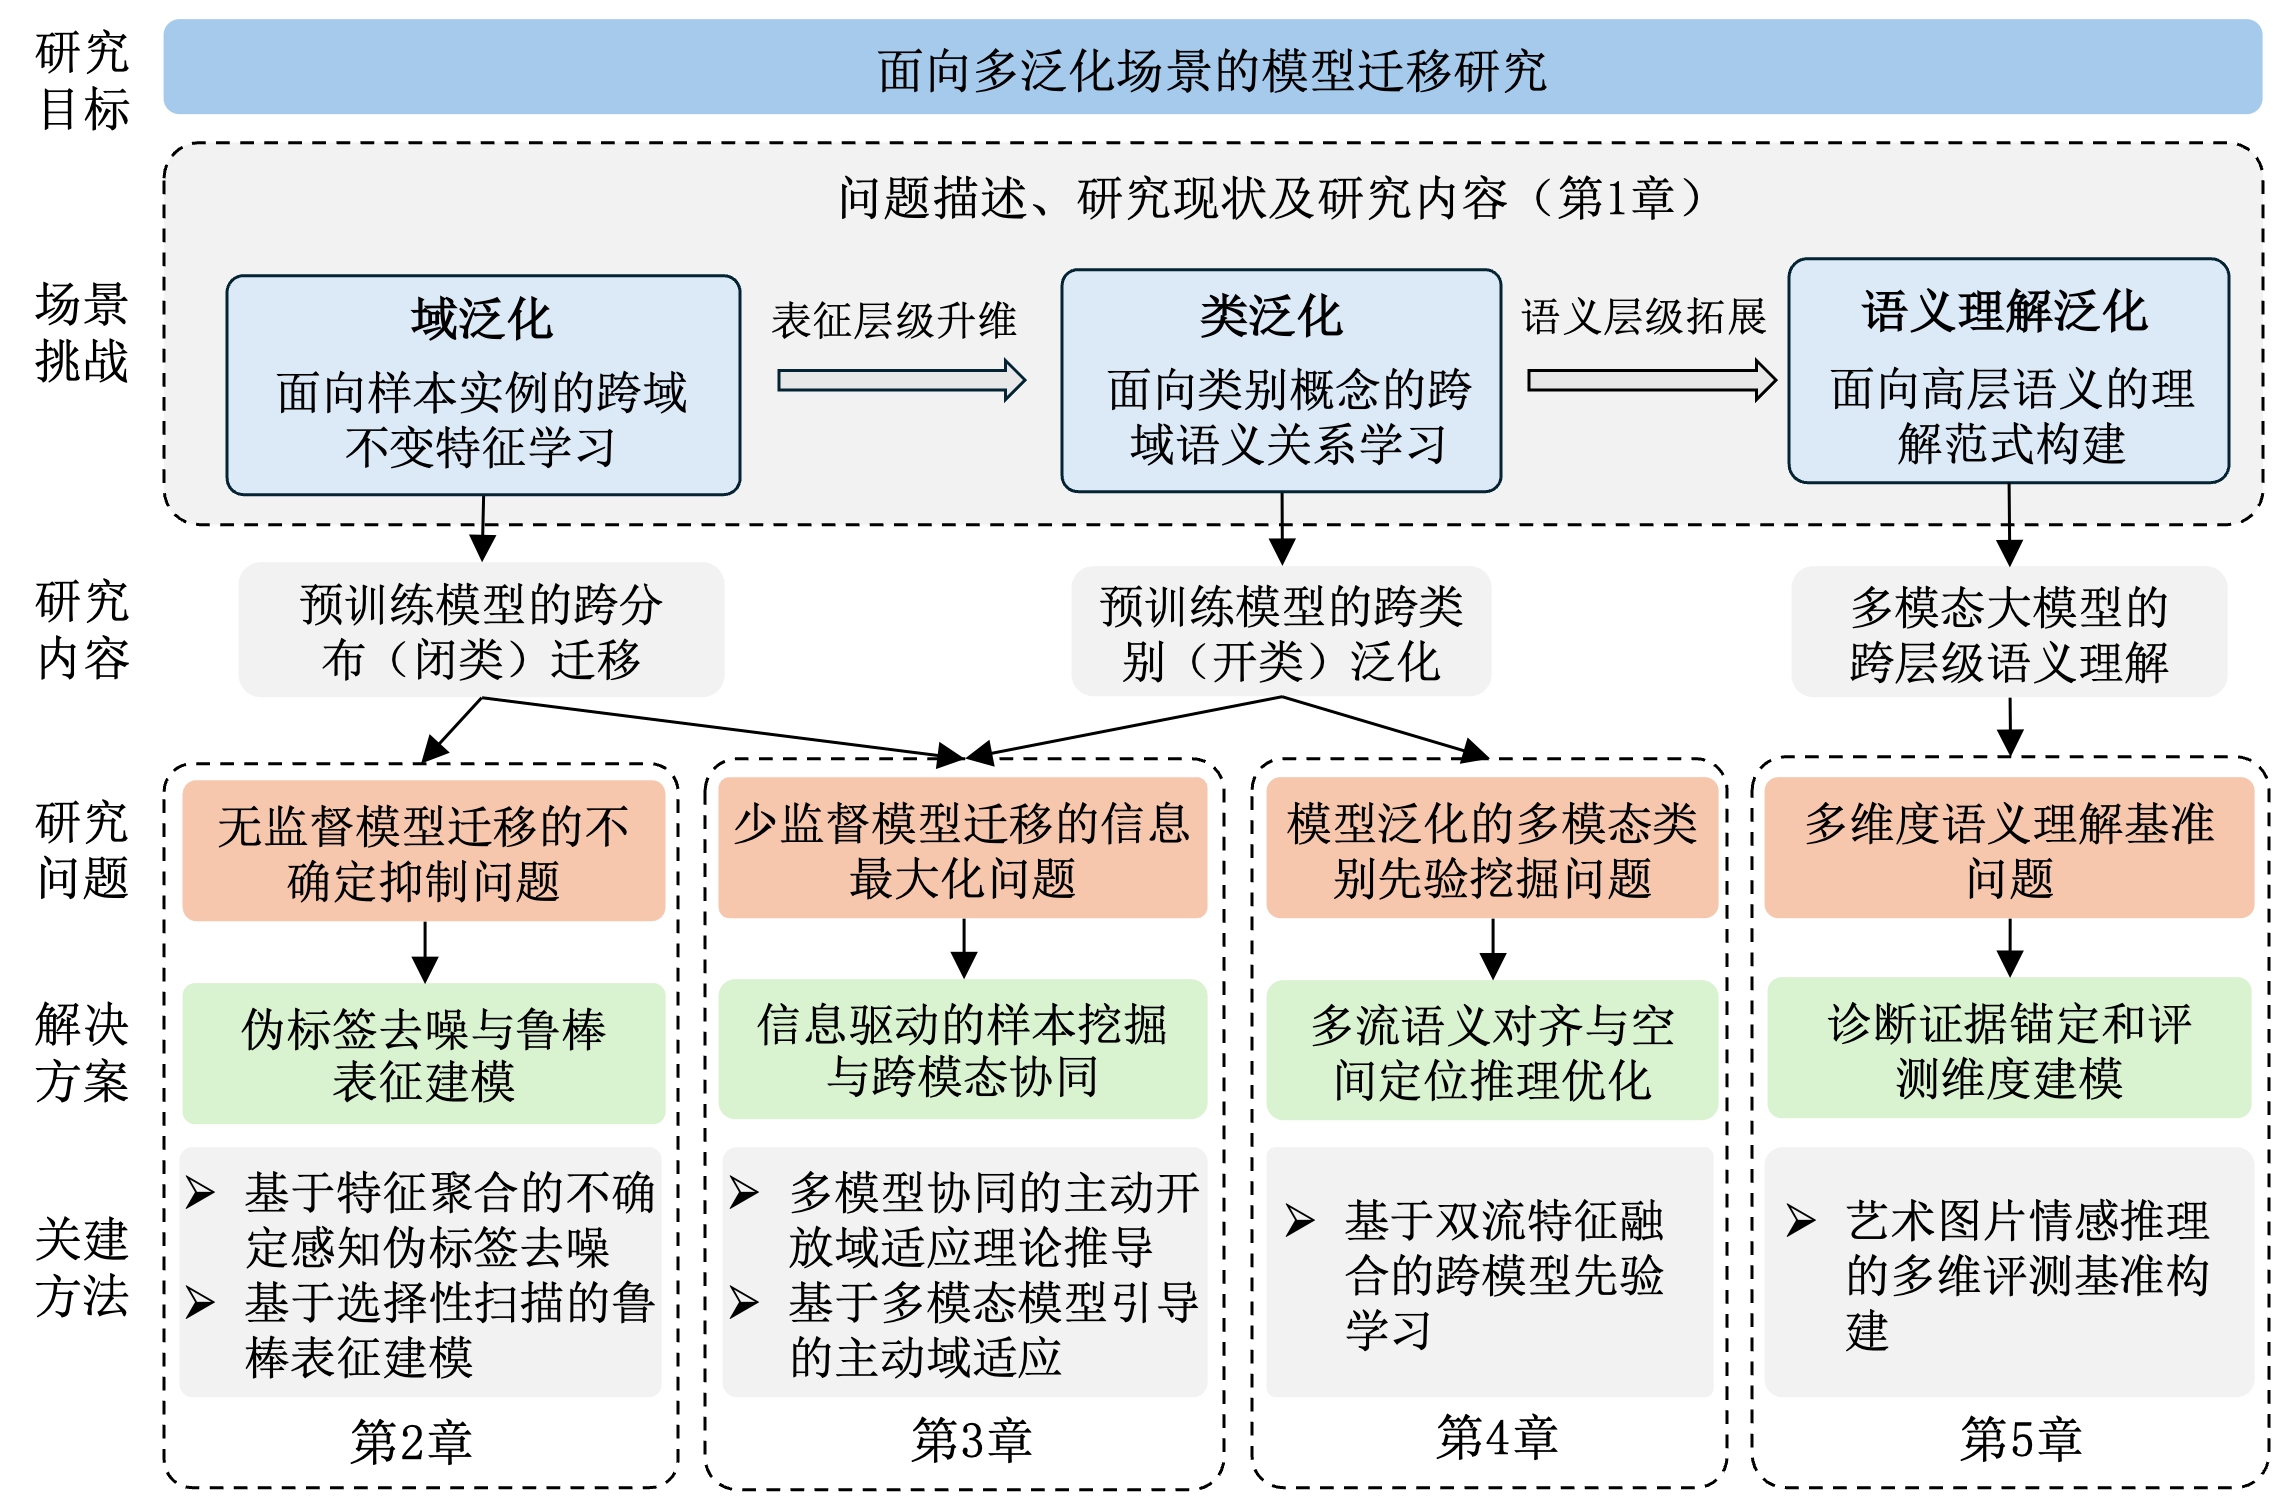
\includegraphics[width=1.\textwidth]{figures/frame.png}
 \bicaption[fig:research_map]{}{面向多泛化场景的模型迁移研究框架}{Fig.}{Research framework of model transfer across multiple generalization scenarios.}
\end{figure}


本文的研究目标是面向多泛化场景的模型迁移研究。如图~\ref{fig:research_map}所示，本文以数据分布、类别词表和语义层次的变化为主线，将研究内容组织为域泛化、类泛化和语义理解泛化三个递进层次。三个层次分别对应预训练模型的跨分布闭类迁移、跨类别开类泛化，以及多模态大语言模型的跨层级语义理解。
% 本文主要研究内容及各章节关系如图~\ref{fig:research_map}所示。

首先，面向跨域泛化这种面向样本示例的跨域不变特征学习，针对无监督模型迁移的不确定性抑制问题，对无源域适应中伪标签噪声与表征虚假相关性两类不确定性来源，按不确定性的作用层次协同开展研究。针对判别层的样本伪标签噪声这一迁移不确定性的主要载体，提出基于特征聚合的不确定性感知伪标签去噪方法 UPA，估计样本级不确定性以自适应筛选高质量伪标签、并抑制噪声标签的记忆传播；针对鲁棒表征建模问题，提出基于选择性扫描的不确定性感知迁移方法 SfMamba，通过跨通道频率域增强与语义一致性打乱策略抑制跨域迁移中的虚假相关性累积，两者在统一自训练框架下协同抑制迁移不确定性；
在此基础上，面向稀缺标注预算下跨模型协同监督不足的问题，针对源模型与视觉—语言模型假设空间层面的信息对齐与知识迁移问题，提出基于多模态基础模型引导的双主动域适应方法 DAMF，将视觉—语言模型作为目标样本与源假设空间之间的互补语义监督信号，通过双聚焦样本选择与交替蒸馏实现两类模型在开放集假设空间的双向深度协同。

面向跨类泛化这种面向类别概念的跨语义关系学习，首先针对开放集无源域适应中已知类别与未知类别难以同时兼顾的问题，利用视觉—语言模型在自然语言空间的零样本识别能力指导目标域已知类的判别建模，进一步通过不确定性感知的开放集校准机制实现对未知类别样本的可靠识别；其次针对开放词汇分割中掩码质量与类别语义识别之间的错配问题，视觉定位模型擅长像素级定位但缺乏语义泛化能力、语义—语言模型具备零样本识别能力但特征空间偏全局且边界粗糙，提出跨模型先验融合的开放词汇分割方法 CMPF，将定位模型的空间先验与语义模型的类别先验在统一解码框架内交叉融合，实现对未见类别的稳定识别。

进一步的，面向多模态多维度的情感评测的标准构建需求，针对多维度语义理解标准制定问题，构建AER-Bench，建立从低层视觉线索到高层情感推理的结构化诊断框架，将艺术情感理解拆解为感知维度、情感与 VAD、基于证据的推理、情感描述四个互补层级并模板化生成单图/配对结构化题目，通过确定性指标与基于大语言模型的细粒度评分相结合的混合协议，对代表性多模态大语言模型在艺术情感推理上的能力进行系统评测，揭示其在视觉证据锚定、感知—情感映射与情感解释一致性上的系统性缺陷。

相关研究由域泛化、类泛化到语义理解泛化三个维度依次推进，并在表征层级升维与语义层级拓展的驱动下形成完整的模型迁移研究体系。
% Local Variables:
% TeX-master: "../thesis"
% TeX-engine: xetex
% End:
